% Provenance (never printed): see sources/outline_sources.md (Year 3:
% dislocation and diffusion creep; flow laws; deformation maps; shear zones and
% kinematic indicators). Brief: sources/book5/BRIEFS.md, ch. 7. Curves from
% figdata/bachelor-3/flow_laws.py. Exercise and problem values in the Book 5
% scratch calculator calc/ch07.py.
\chapter{Deformation Mechanisms and Shear Zones}\label{ch:b3:deformation-mechanisms}

At the surface, the granite of a mountain shatters along faults. Twenty
kilometres down, the same granite flows like toffee in a \omterm{def:b3:deformation-mechanisms:shear-zone}{shear zone} a few
hundred metres wide, its feldspars rolled into eyes and its quartz drawn out
into ribbons. A crystal can flow without breaking because it is never perfect:
it moves by its defects, one row of atoms at a time, or by atoms diffusing from
one face of a grain to another. This chapter follows those mechanisms from the
crystal lattice to the laws that geodynamics uses, to the maps that say which
mechanism wins, and to the \omterm{def:b3:deformation-mechanisms:shear-zone}{shear zones} in which the rock records how it moved.

\begin{recall}
Point defects, the Arrhenius law and the activation energy are in the
chemistry books' university volumes; the diffusion coefficient in the physics
books'. Stress and strain, the strain ellipse, simple shear and its ellipse
($S_{1,2} = \sqrt{1 + \gamma^2/4} \pm \gamma/2$, long axis at $\theta'$ from the
shear direction with $\tan2\theta' = 2/\gamma$), power-law creep with its
constants for wet quartzite and dry olivine, the strength envelope and the
brittle--ductile transition are in the Year 1 volume, in its chapter on
stress, strain and rheology; foliation, lineation and the descriptive
mylonite in its chapter on faults, folds and fabrics. The effective viscosity
of the mantle is in \cref{ch:b3:mantle-convection}.
\end{recall}

\section{Crystal defects}

To shear a perfect crystal, every bond across a lattice plane would have to
break at once, and that needs a stress of the order of a tenth of the shear
modulus, which in the mantle is about \qty{8e10}{Pa}
(\cref{ch:b3:mantle-convection}): thousands of megapascals. Real crystals
yield at far lower stresses, because they slip one line of atoms at a time.

\begin{definition}[Dislocation]\label{def:b3:deformation-mechanisms:dislocation}
A \emph{dislocation}\index{dislocation (crystal defect)} is a line defect in a
crystal: the boundary, inside the crystal, between a part of a lattice plane
that has slipped and a part that has not. Its \emph{Burgers vector}
$\mathbf b$ is the slip that it carries, one lattice spacing in a lattice
direction. In an edge dislocation $\mathbf b$ is perpendicular to the line,
which is the edge of an extra half-plane of atoms; in a screw dislocation it
is parallel to the line. A dislocation moves by \emph{glide} on its slip plane,
and an edge dislocation leaves that plane by \emph{climb}, as atoms or
vacancies diffuse to or from the edge of its half-plane.
\end{definition}

\begin{omfigure}
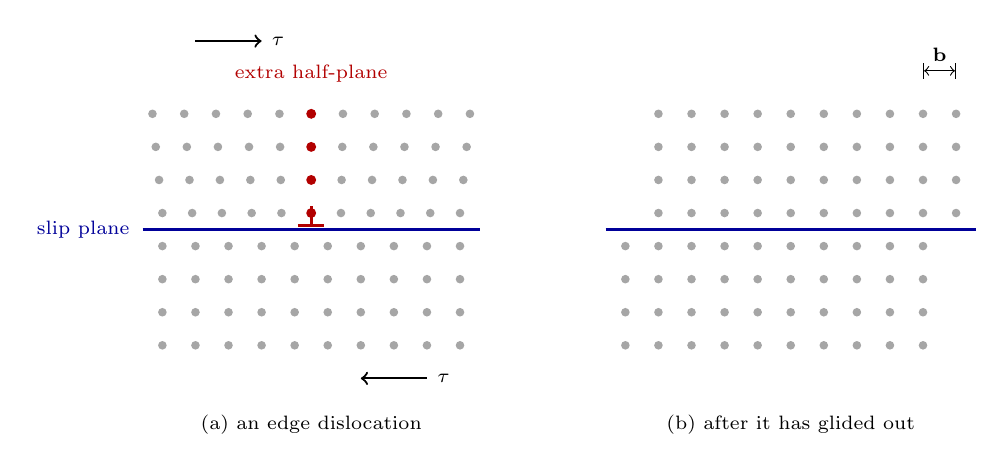
\begin{tikzpicture}[font=\scriptsize, x=0.42cm, y=0.42cm]
% (a) lower half: 10 columns; upper half: 11 columns squeezed over the same width
\foreach \j in {0,...,3} {\foreach \i in {0,...,9} {\fill[gray!70] (\i,\j) circle (0.13);}}
\foreach \j/\s in {4/0.9, 5/0.92, 6/0.94, 7/0.96} {\foreach \i in {0,...,10} {
  \pgfmathsetmacro{\x}{(\i-5)*\s + 4.5}
  \ifnum\i=5 \fill[red!70!black] (\x,\j) circle (0.15); \else \fill[gray!70] (\x,\j) circle (0.13); \fi}}
\draw[thick, blue!60!black] (-0.6,3.5) -- (9.6,3.5);
\node[anchor=east, blue!60!black] at (-0.7,3.5) {slip plane};
\draw[red!70!black, very thick] (4.1,3.62) -- (4.9,3.62) (4.5,3.62) -- (4.5,4.2);
\node[red!70!black] at (4.5,8.2) {extra half-plane};
\draw[->, thick] (1.0,9.2) -- (3.0,9.2) node[right] {$\tau$};
\draw[<-, thick] (6.0,-1.0) -- (8.0,-1.0) node[right] {$\tau$};
% (b) after glide: the upper half shifted by one spacing
\begin{scope}[shift={(14,0)}]
\foreach \j in {0,...,3} {\foreach \i in {0,...,9} {\fill[gray!70] (\i,\j) circle (0.13);}}
\foreach \j in {4,...,7} {\foreach \i in {1,...,10} {\fill[gray!70] (\i,\j) circle (0.13);}}
\draw[thick, blue!60!black] (-0.6,3.5) -- (10.6,3.5);
\draw[|<->|] (9,8.3) -- (10,8.3) node[midway, above] {$\mathbf b$};
\end{scope}
\node[anchor=north] at (4.5,-1.8) {(a) an edge dislocation};
\node[anchor=north] at (19,-1.8) {(b) after it has glided out};
\end{tikzpicture}

\par\smallskip{\small (a) An edge \omterm{def:b3:deformation-mechanisms:dislocation}{dislocation}: an extra half-plane of atoms (red)
ends on the slip plane, distorting the lattice around its edge (the symbol
$\perp$). Under the shear stress $\tau$ it glides along the slip plane by
breaking and re-forming one row of bonds at a time. (b) When it has crossed the
crystal, the upper half has slipped by one Burgers vector $\mathbf b$, and the
lattice is perfect again.}\label{fig:b3:deformation-mechanisms:dislocation}
\end{omfigure}

The lattice resists the glide of a \omterm{def:b3:deformation-mechanisms:dislocation}{dislocation} with a small stress, the
Peierls stress, which depends on the strength and the direction of the bonds:
that is why some slip systems of a mineral are easy and others hard. As a
crystal deforms, \omterm{def:b3:deformation-mechanisms:dislocation}{dislocations} multiply and tangle; they block one another, and
the crystal hardens, unless they can climb round obstacles or annihilate, which
needs diffusion, hence heat.

\section{Mechanisms of creep}

\begin{definition}[Mechanisms of creep]\label{def:b3:deformation-mechanisms:creep}
In \emph{dislocation creep}\index{dislocation creep} crystals deform by the
glide of \omterm{def:b3:deformation-mechanisms:dislocation}{dislocations}, with climb releasing them from obstacles. In
\emph{diffusion creep}\index{diffusion creep} they change shape by the
diffusion of atoms, through the lattice (Nabarro--Herring creep) or along the
grain boundaries (Coble creep), from the faces under the highest normal stress
to those under the lowest. In \emph{grain-boundary sliding}\index{grain-boundary
sliding} grains slide past one another along their boundaries, the gaps being
closed by diffusion or \omterm{def:b3:deformation-mechanisms:dislocation}{dislocation} creep. In \emph{pressure
solution}\index{pressure solution} the matter dissolves in a fluid film on the
faces under high stress and is deposited where the stress is low, or carried
away.
\end{definition}

\begin{proposition}[Grain-size dependence of diffusion creep]\label{prop:b3:deformation-mechanisms:grain-size}
At low stress $\sigma$, a rock of grain size $d$ creeps by diffusion at the rate
\[
  \dot\varepsilon \approx B_L\frac{D_L\Omega}{k_BT}\frac{\sigma}{d^2}
  \quad\text{(through the lattice)},\qquad
  \dot\varepsilon \approx B_B\frac{\delta D_B\Omega}{k_BT}\frac{\sigma}{d^3}
  \quad\text{(along the boundaries)},
\]
where $D_L$ and $D_B$ are the diffusion coefficients in the lattice and in the
boundaries, $\delta$ the width of a boundary, $\Omega$ the volume of an atom,
$k_B$ Boltzmann's constant and $B_L$, $B_B$ numbers of order ten that depend on
the shape of the grains.
\end{proposition}

\begin{proof}
A normal stress $\sigma$ on a face changes the work needed to form a vacancy
there by $\sigma\Omega$, so the concentration $C$ of vacancies differs between
faces under tension and under compression by $\Delta C \approx C\sigma\Omega/
(k_BT)$ when $\sigma\Omega \ll k_BT$. Across a distance of order $d$, the
diffusive flux of vacancies, hence of atoms the other way, is of order $D\Delta
C/d$ per unit area. Through the lattice the flux crosses an area of order
$d^2$, along the boundaries an area of order $\delta d$. The volume moved per
unit time, divided by the grain's volume $d^3$, is the strain rate: of order
$(D_L\sigma\Omega/k_BT)\,d^2/(d\cdot d^3) = D_L\sigma\Omega/(k_BTd^2)$ in the
lattice, and $(D_B\sigma\Omega/k_BT)\,\delta d/(d\cdot d^3) = \delta D_B
\sigma\Omega/(k_BTd^3)$ in the boundaries. The product $C\,D$ is the
self-diffusion coefficient written $D$ in the statement.
\end{proof}

\omterm{def:b3:deformation-mechanisms:creep}{Diffusion creep} is linear in the stress, a true viscous flow, and it is fast in
fine-grained rock: halving the grain size makes Coble creep eight times faster
(figure below). \omterm{def:b3:deformation-mechanisms:creep}{Dislocation creep} does not depend on the grain size, but grows
with a high power of the stress.

\begin{omfigure}
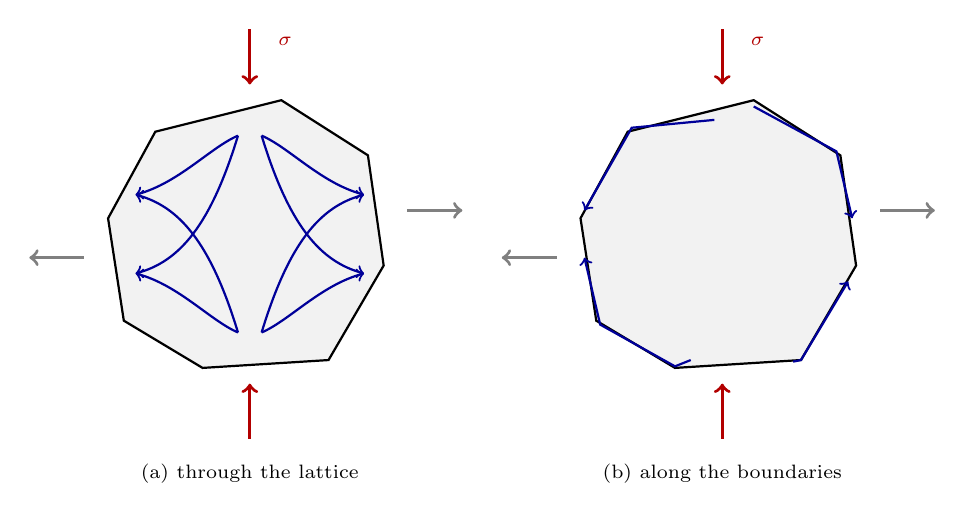
\begin{tikzpicture}[font=\scriptsize, x=1cm, y=1cm]
\foreach \cx/\lab in {0/{(a) through the lattice}, 6/{(b) along the boundaries}} {
  \begin{scope}[shift={(\cx,0)}]
  \draw[thick, fill=gray!10] (-1.6,-1.1) -- (-0.6,-1.7) -- (1.0,-1.6) -- (1.7,-0.4) -- (1.5,1.0) -- (0.4,1.7) -- (-1.2,1.3) -- (-1.8,0.2) -- cycle;
  \draw[->, very thick, red!70!black] (0,2.6) -- (0,1.9);
  \draw[->, very thick, red!70!black] (0,-2.6) -- (0,-1.9);
  \node[red!70!black] at (0.45,2.45) {$\sigma$};
  \draw[<-, very thick, gray] (2.7,0.3) -- (2.0,0.3);
  \draw[<-, very thick, gray] (-2.8,-0.3) -- (-2.1,-0.3);
  \node[anchor=north] at (0,-2.8) {\lab};
  \end{scope}
}
\foreach \sx in {1,-1} {\foreach \y in {-0.5,0.5} {
  \draw[->, blue!60!black, thick] (0.15*\sx,1.25) .. controls (0.5*\sx,\y+0.6) and (0.9*\sx,\y+0.15) .. (1.45*\sx,\y);
  \draw[->, blue!60!black, thick] (0.15*\sx,-1.25) .. controls (0.5*\sx,\y-0.6) and (0.9*\sx,\y-0.15) .. (1.45*\sx,\y);
}}
\draw[->, blue!60!black, thick] (6.4,1.62) -- (7.45,1.05) -- (7.65,0.2);
\draw[->, blue!60!black, thick] (5.9,1.45) -- (4.85,1.35) -- (4.25,0.3);
\draw[->, blue!60!black, thick] (6.9,-1.62) -- (7.0,-1.6) -- (7.6,-0.6);
\draw[->, blue!60!black, thick] (5.6,-1.6) -- (5.4,-1.68) -- (4.45,-1.15) -- (4.25,-0.3);
\end{tikzpicture}

\par\smallskip{\small \omterm{def:b3:deformation-mechanisms:creep}{Diffusion creep} of a grain shortened along $\sigma$. Atoms
leave the faces under the highest compression and are added to the faces under
the lowest (blue), so the grain flattens and lengthens (grey arrows): (a)
through the grain's interior, Nabarro--Herring creep; (b) along its boundaries,
Coble creep.}\label{fig:b3:deformation-mechanisms:diffusion}
\end{omfigure}

Deformed crystals also mend themselves while they deform.

\begin{definition}[Recovery, subgrain, dynamic recrystallisation]\label{def:b3:deformation-mechanisms:recrystallisation}
\emph{Recovery}\index{recovery (crystal plasticity)} is the rearrangement of
\omterm{def:b3:deformation-mechanisms:dislocation}{dislocations}, by climb and cross-slip, into lower-energy arrays, and their
annihilation. \omterm{def:b3:deformation-mechanisms:dislocation}{Dislocations} arranged in walls divide a grain into
\emph{subgrains}\index{subgrain}, parts of the grain whose lattices are tilted
by a few degrees from one another. \emph{Dynamic
recrystallisation}\index{dynamic recrystallisation} is the replacement, during
deformation, of strained grains by new grains with fewer \omterm{def:b3:deformation-mechanisms:dislocation}{dislocations}, either
by the rotation of subgrains until they become grains, or by the migration of
grain boundaries into the more strained neighbours.
\end{definition}

\begin{definition}[Crystallographic preferred orientation]\label{def:b3:deformation-mechanisms:cpo}
A rock has a \emph{crystallographic preferred orientation}\index{crystallographic
preferred orientation} (CPO) when the lattices of its grains are not oriented
at random but cluster about directions set by the deformation; \omterm{def:b3:deformation-mechanisms:creep}{dislocation
creep} produces it, by rotating each grain's slip systems towards the flow.
\end{definition}

A rock with a CPO inherits the anisotropy of its crystals: its seismic speeds,
for instance, depend on direction, which lets seismology see the fabric of
the deep mantle. \omterm{def:b3:deformation-mechanisms:creep}{Diffusion creep} and \omterm{def:b3:deformation-mechanisms:creep}{grain-boundary sliding}, which let grains
rotate freely, do not build one.

\section{Flow laws}

\begin{definition}[Flow law, stress exponent, homologous temperature]\label{def:b3:deformation-mechanisms:flow-law}
A \emph{flow law}\index{flow law} gives the strain rate of a rock deforming by
one mechanism as a function of the differential stress $\sigma$, the grain size
$d$, the temperature $T$ and the pressure $P$:
\[
  \dot\varepsilon = A\,\sigma^nd^{-m}\exp\Bigl(-\frac{E + PV}{RT}\Bigr),
\]
with $A$, $n$, $m$, the activation energy $E$ and the activation volume $V$
measured in the laboratory. The \emph{stress exponent}\index{stress exponent}
is $n$, the grain-size exponent $m$. The \emph{homologous
temperature}\index{homologous temperature} of a mineral is $T/T_m$, its
absolute temperature over its absolute melting temperature.
\end{definition}

In the laws used here, \omterm{def:b3:deformation-mechanisms:creep}{dislocation creep} has $n$ of 3.5 or 4 and $m = 0$;
\omterm{def:b3:deformation-mechanisms:creep}{diffusion creep} has $n = 1$ and $m = 2$ or 3 (\cref{prop:b3:deformation-mechanisms:grain-size}).
Creep grows as the \omterm{def:b3:deformation-mechanisms:flow-law}{homologous temperature} approaches 1. Forsterite melts at \qty{1890}{\celsius}, so the mantle at \qty{1300}{\celsius}
stands at $T/T_m = 0.73$; ice at \qty{-10}{\celsius} at 0.96, which is why
glaciers flow. The olivine values used here are those of a widely used
laboratory compilation: dry olivine in \omterm{def:b3:deformation-mechanisms:creep}{dislocation creep}, $A =
\num{1.1e5}$, $n = 3.5$, $E = \qty{530}{kJ.mol^{-1}}$, $V =
\qty{14}{cm^3.mol^{-1}}$; in \omterm{def:b3:deformation-mechanisms:creep}{diffusion creep}, $A = 10^{9.2}$, $n = 1$, $m = 3$,
$E = \qty{375}{kJ.mol^{-1}}$, $V = \qty{5}{cm^3.mol^{-1}}$ (stress in megapascals,
grain size in micrometres, time in seconds); wet quartzite is the Year 1
volume's. Water weakens olivine: at a water fugacity of about
\qty{300}{MPa}, olivine aggregates creep five to six times faster than dry ones
in \omterm{def:b3:deformation-mechanisms:creep}{dislocation creep}, five times faster in \omterm{def:b3:deformation-mechanisms:creep}{diffusion creep}.
% ledger: bowen14:mgo-sio2, azuma17:olivine, lopez:flow-laws, codata:R, mk00:diffusion, mk00:dislocation

\begin{proposition}[Effective viscosity]\label{prop:b3:deformation-mechanisms:viscosity}
A rock obeying a \omterm{def:b3:deformation-mechanisms:flow-law}{flow law} $\dot\varepsilon = A'\sigma^n$ at given $T$, $P$ and
$d$ has the effective viscosity
\[
  \eta_{\mathrm{eff}} = \frac{\sigma}{2\dot\varepsilon}
  = \tfrac12A'^{-1/n}\,\dot\varepsilon^{(1-n)/n}:
\]
for $n > 1$ it falls as the rock deforms faster.
\end{proposition}

\begin{proof}
For a Newtonian fluid, $\sigma = 2\eta\dot\varepsilon$ in a uniaxial flow, by the
definition of viscosity; $\eta_{\mathrm{eff}}$ is the viscosity of the Newtonian
fluid that would flow at the same rate under the same stress. Substituting
$\sigma = (\dot\varepsilon/A')^{1/n}$ gives the second form.
\end{proof}

Wet quartzite at \qty{400}{\celsius} flowing at \qty{e-14}{s^{-1}} needs
\qty{65}{MPa} and has an effective viscosity of \qty{3.3e21}{Pa.s}; at
\qty{500}{\celsius}, \qty{18}{MPa} and \qty{9e20}{Pa.s}: a hundred degrees
divides the strength by more than three (figure below). Dry olivine at
\qty{1100}{\celsius} and \qty{1}{GPa} needs only \qty{3}{MPa}. The strength
envelopes of the Year 1 volume are built from exactly these laws.

\begin{omfigure}
\begin{tikzpicture}
\begin{groupplot}[group style={group size=2 by 1, horizontal sep=1.6cm},
  omrecord, width=0.47\linewidth, height=0.47\linewidth, xmode=log,
  xmin=1, xmax=1000, ymin=-20, ymax=-6, xlabel={differential stress (MPa)},
  legend style={font=\scriptsize, at={(0.97,0.03)}, anchor=south east, legend columns=1}]
\nextgroupplot[ylabel={$\log_{10}\dot\varepsilon$ (\unit{s^{-1}})}, title={(a) wet quartzite},
  title style={font=\small}]
% computed in figdata/bachelor-3/flow_laws.py; ledger: lopez:flow-laws, azuma17:olivine
\addplot[omDef, thick] table[x=s, y=r600] {figdata/out/bachelor-3-flow_laws-quartz.dat};
\addlegendentry{\qty{600}{\celsius}}
\addplot[red!70!black, thick, densely dashed] table[x=s, y=r500] {figdata/out/bachelor-3-flow_laws-quartz.dat};
\addlegendentry{\qty{500}{\celsius}}
\addplot[black, thick, densely dotted] table[x=s, y=r400] {figdata/out/bachelor-3-flow_laws-quartz.dat};
\addlegendentry{\qty{400}{\celsius}}
\draw[gray] (axis cs:1,-14) -- (axis cs:1000,-14);
\nextgroupplot[title={(b) dry olivine, \qty{1}{GPa}}, title style={font=\small}]
\addplot[omDef, thick] table[x=s, y=r1300] {figdata/out/bachelor-3-flow_laws-olivine.dat};
\addlegendentry{\qty{1300}{\celsius}}
\addplot[red!70!black, thick, densely dashed] table[x=s, y=r1100] {figdata/out/bachelor-3-flow_laws-olivine.dat};
\addlegendentry{\qty{1100}{\celsius}}
\addplot[black, thick, densely dotted] table[x=s, y=r900] {figdata/out/bachelor-3-flow_laws-olivine.dat};
\addlegendentry{\qty{900}{\celsius}}
\draw[gray] (axis cs:1,-14) -- (axis cs:1000,-14);
\end{groupplot}
\end{tikzpicture}

\par\smallskip{\small Dislocation-creep \omterm{def:b3:deformation-mechanisms:flow-law}{flow laws}: strain rate against stress at
three temperatures. The slope on these axes is the \omterm{def:b3:deformation-mechanisms:flow-law}{stress exponent}, 4 for
quartzite and 3.5 for olivine; the grey line marks a geological strain rate,
\qty{e-14}{s^{-1}}. Olivine needs temperatures some \qty{600}{\celsius} higher
than quartz to flow as easily.}\label{fig:b3:deformation-mechanisms:flow-laws}
\end{omfigure}

\section{Deformation mechanism maps}

Several mechanisms run in parallel, and the fastest carries the deformation.

\begin{definition}[Deformation mechanism map]\label{def:b3:deformation-mechanisms:deformation-map}
A \emph{deformation mechanism map}\index{deformation mechanism map} of a
mineral or rock shows, on axes of two of the variables stress, grain size and
temperature, the fields in which each mechanism is the fastest, with contours
of the total strain rate.
\end{definition}

\begin{proposition}[Mechanism boundary]\label{prop:b3:deformation-mechanisms:boundary}
At given $T$ and $P$, \omterm{def:b3:deformation-mechanisms:creep}{dislocation creep} ($A_1$, $n_1$, $E_1$, $V_1$, no
grain-size dependence) and \omterm{def:b3:deformation-mechanisms:creep}{diffusion creep} ($A_2$, $n_2 = 1$, $m$, $E_2$, $V_2$)
run equally fast at the stress
\[
  \sigma_b = \biggl(\frac{A_2d^{-m}}{A_1}
  \exp\frac{(E_1 - E_2) + P(V_1 - V_2)}{RT}\biggr)^{1/(n_1 - 1)} ,
\]
so the boundary is a straight line of slope $-m/(n_1 - 1)$ on logarithmic
axes of grain size and stress; \omterm{def:b3:deformation-mechanisms:creep}{dislocation creep} wins above it.
\end{proposition}

\begin{proof}
Equate the two \omterm{def:b3:deformation-mechanisms:flow-law}{flow laws} and solve for $\sigma$. Above $\sigma_b$, the ratio of
the two rates, proportional to $\sigma^{n_1 - 1}$, exceeds 1.
\end{proof}

For dry olivine at \qty{1100}{\celsius} and \qty{2}{GPa}, the boundary lies at
\qty{5}{MPa} for a grain size of \qty{1}{mm} and at \qty{79}{MPa} for
\qty{100}{\micro m} (figure below). Fine-grained mantle creeps by diffusion,
coarse mantle by \omterm{def:b3:deformation-mechanisms:dislocation}{dislocations}; laboratory and geophysical evidence suggests
that both regimes occur in the upper mantle, the hot, shallow mantle flowing by
\omterm{def:b3:deformation-mechanisms:creep}{dislocation creep} and the colder or deeper by \omterm{def:b3:deformation-mechanisms:creep}{diffusion creep}, and that where
the stress rises and the grains shrink, the mantle near the boundary weakens
and the deformation localises.
% ledger: azuma17:olivine, karato93:transitions

\begin{omfigure}
\begin{tikzpicture}
\begin{axis}[omrecord, xmode=log, ymode=log, width=0.78\linewidth, height=0.58\linewidth,
  xmin=10, xmax=1e4, ymin=0.01, ymax=1000, xlabel={grain size (\unit{\micro m})},
  ylabel={differential stress (MPa)}, clip=true]
% computed in figdata/bachelor-3/flow_laws.py; ledger: azuma17:olivine
\addplot[black, very thick] table[x=d, y=s] {figdata/out/bachelor-3-flow_laws-mapbound.dat};
\foreach \c in {16,14,12,10} {
  \addplot[omDef, thick] table[x=d, y=s\c] {figdata/out/bachelor-3-flow_laws-mapcont.dat};
}
\node[font=\scriptsize, fill=white, inner sep=1pt] at (axis cs:7000,1.15) {$10^{-16}$};
\node[font=\scriptsize, fill=white, inner sep=1pt] at (axis cs:7000,4.2) {$10^{-14}$};
\node[font=\scriptsize, fill=white, inner sep=1pt] at (axis cs:7000,15.7) {$10^{-12}$};
\node[font=\scriptsize, fill=white, inner sep=1pt] at (axis cs:4200,58) {$10^{-10}\,\unit{s^{-1}}$};
\node[font=\small, anchor=north east] at (axis cs:9000,600) {dislocation creep};
\node[font=\small, anchor=south west] at (axis cs:1500,0.013) {diffusion creep};
\end{axis}
\end{tikzpicture}

\par\smallskip{\small \omterm{def:b3:deformation-mechanisms:deformation-map}{Deformation mechanism map} of dry olivine at
\qty{1100}{\celsius} and \qty{2}{GPa}. The thick line divides the fields where
\omterm{def:b3:deformation-mechanisms:creep}{dislocation creep} (above) and \omterm{def:b3:deformation-mechanisms:creep}{diffusion creep} (below) is faster; the thin lines
are contours of the total strain rate, flat where \omterm{def:b3:deformation-mechanisms:creep}{dislocation creep}, which
ignores the grain size, dominates.}\label{fig:b3:deformation-mechanisms:map}
\end{omfigure}

The grain size that \omterm{def:b3:deformation-mechanisms:recrystallisation}{dynamic recrystallisation} produces depends on the stress,
and this makes the grains a stress gauge.

\begin{definition}[Palaeopiezometer]\label{def:b3:deformation-mechanisms:piezometer}
A \emph{palaeopiezometer}\index{palaeopiezometer} is a feature of a deformed
rock whose size or density is set by the differential stress under which it
formed, calibrated in the laboratory, from which the stress of a past
deformation can be read.
\end{definition}

For quartz, experiments at \qty{1.5}{GPa} and 800 to \qty{1100}{\celsius}, at
flow stresses from 34 to \qty{268}{MPa}, gave recrystallised grains from 46 down
to \qty{3.2}{\micro m}, fitted by
\[
  D = 10^{3.56}\,\sigma^{-1.26}\qquad(D\text{ in \unit{\micro m}},\ \sigma\text{ in MPa}),
\]
with no detectable effect of the temperature. A quartz mylonite with
recrystallised grains \qty{20}{\micro m} across deformed under about
\qty{62}{MPa}.
% ledger: st03:piezometer

\section{Shear zones}

\begin{definition}[Shear zone, strain softening]\label{def:b3:deformation-mechanisms:shear-zone}
A \emph{shear zone}\index{shear zone} is a tabular zone, between walls that are
little deformed, in which the strain is concentrated and is close to a simple
shear parallel to the zone. A rock undergoes \emph{strain
softening}\index{strain softening} when its strength falls as it deforms.
\end{definition}

\omterm{def:b3:deformation-mechanisms:shear-zone}{Strain softening} is what keeps a \omterm{def:b3:deformation-mechanisms:shear-zone}{shear zone} narrow: once a band is weaker
than its walls, the deformation stays in it. Grain-size reduction by \omterm{def:b3:deformation-mechanisms:recrystallisation}{dynamic
recrystallisation}, which may tip the rock into \omterm{def:b3:deformation-mechanisms:creep}{diffusion creep}, the growth of a
CPO that aligns easy slip systems, the entry of water and reactions that make
weak minerals such as micas all soften the rock. The mylonites of the Year 1
volume are their product. In a \omterm{def:b3:deformation-mechanisms:shear-zone}{shear zone} of simple shear, a marker that
crossed the zone at right angles is deflected into it: if inside the zone it
makes the angle $\psi$ with its original direction, the shear strain is $\gamma
= \tan\psi$, and the displacement across a zone of width $w$ is $\gamma w$.

\begin{definition}[Kinematic indicators]\label{def:b3:deformation-mechanisms:kinematic}
A \emph{kinematic indicator}\index{kinematic indicator} is a structure whose
asymmetry records the \emph{sense of shear}\index{sense of shear}, the sense in
which one wall of a \omterm{def:b3:deformation-mechanisms:shear-zone}{shear zone} moved relative to the other, read in the plane
that contains the stretching lineation and is perpendicular to the foliation.
An \emph{S--C fabric}\index{S--C fabric} is a pair of foliations: S, the
foliation of flattened grains, oblique to the zone and turned towards the
direction of stretching, and C, shear bands parallel to the zone. A
\emph{porphyroclast system}\index{porphyroclast system} is a strong grain with
tails of recrystallised material: in a $\sigma$-type the tails step from one
side of the clast's centre line to the other without crossing it, in a
$\delta$-type, dragged round by the clast's rotation, they cross it. A
\emph{mica fish}\index{mica fish} is a lozenge-shaped mica grain inclined to
the shear plane, with thin tails, stepping like those of a $\sigma$-type clast.
\end{definition}

\begin{omfigure}
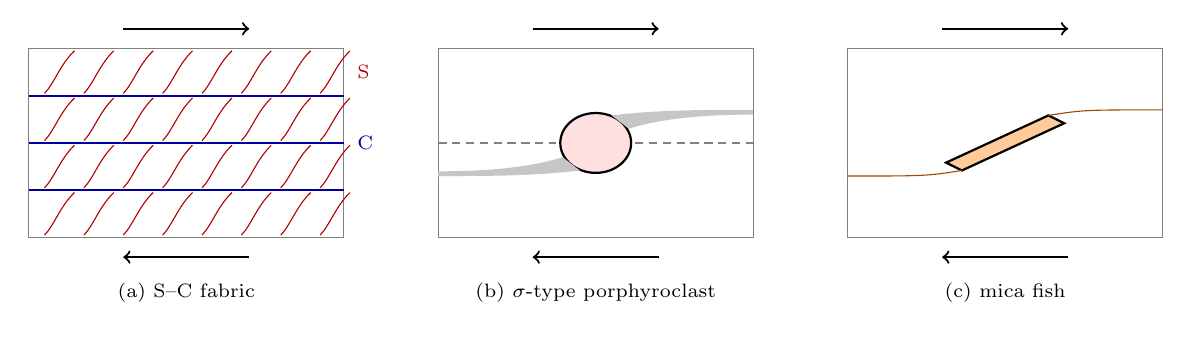
\begin{tikzpicture}[font=\scriptsize, x=1cm, y=1cm]
% (a) S-C fabric, dextral
\begin{scope}
\draw[gray] (0,0) rectangle (4,2.4);
\foreach \y in {0.6,1.2,1.8} {\draw[blue!60!black, thick] (0,\y) -- (4,\y);}
\foreach \y in {0,0.6,1.2,1.8} {\foreach \x in {0.2,0.7,...,3.8} {
  \draw[red!70!black] (\x,\y+0.03) .. controls (\x+0.12,\y+0.15) and (\x+0.2,\y+0.4) .. (\x+0.38,\y+0.57);}}
\draw[->, thick] (1.2,2.65) -- (2.8,2.65);
\draw[<-, thick] (1.2,-0.25) -- (2.8,-0.25);
\node[anchor=north] at (2,-0.45) {(a) S--C fabric};
\node[blue!60!black, anchor=west] at (4.05,1.2) {C};
\node[red!70!black, anchor=west] at (4.05,2.1) {S};
\end{scope}
% (b) sigma clast
\begin{scope}[shift={(5.2,0)}]
\draw[gray] (0,0) rectangle (4,2.4);
\fill[red!12] (2.0,1.2) ellipse (0.45 and 0.38);
\draw[thick] (2.0,1.2) ellipse (0.45 and 0.38);
\fill[gray!45] (2.2,1.55) .. controls (2.8,1.62) and (3.3,1.62) .. (4.0,1.62) -- (4.0,1.56) .. controls (3.3,1.56) and (2.8,1.5) .. (2.42,1.38) -- cycle;
\fill[gray!45] (1.8,0.85) .. controls (1.2,0.78) and (0.7,0.78) .. (0,0.78) -- (0,0.84) .. controls (0.7,0.84) and (1.2,0.9) .. (1.58,1.02) -- cycle;
\draw[gray, densely dashed] (0,1.2) -- (1.5,1.2) (2.5,1.2) -- (4,1.2);
\draw[->, thick] (1.2,2.65) -- (2.8,2.65);
\draw[<-, thick] (1.2,-0.25) -- (2.8,-0.25);
\node[anchor=north] at (2,-0.45) {(b) $\sigma$-type porphyroclast};
\end{scope}
% (c) mica fish
\begin{scope}[shift={(10.4,0)}]
\draw[gray] (0,0) rectangle (4,2.4);
\fill[orange!40] (1.25,0.95) -- (2.55,1.55) -- (2.75,1.45) -- (1.45,0.85) -- cycle;
\draw[thick] (1.25,0.95) -- (2.55,1.55) -- (2.75,1.45) -- (1.45,0.85) -- cycle;
\draw[orange!60!black] (2.55,1.55) .. controls (3.0,1.62) .. (4.0,1.62);
\draw[orange!60!black] (1.45,0.85) .. controls (1.0,0.78) .. (0,0.78);
\draw[->, thick] (1.2,2.65) -- (2.8,2.65);
\draw[<-, thick] (1.2,-0.25) -- (2.8,-0.25);
\node[anchor=north] at (2,-0.45) {(c) mica fish};
\end{scope}
\end{tikzpicture}

\par\smallskip{\small Three \omterm{def:b3:deformation-mechanisms:kinematic}{kinematic indicators} of the same dextral shear
(top to the right, arrows), seen in the plane of the lineation, normal to the
foliation. (a) The S foliation (red) curves into the C shear bands (blue),
leaning in the direction of stretching. (b) The tails of a $\sigma$-type clast
leave its upper side to the right and its lower side to the left, stepping up
in the direction of shear without crossing the centre line (dashed). (c) A
\omterm{def:b3:deformation-mechanisms:kinematic}{mica fish} leans like S, its tails stepping like a $\sigma$-type clast's. Not to
scale.}\label{fig:b3:deformation-mechanisms:kinematic}
\end{omfigure}

Read together, a few indicators that agree give the \omterm{def:b3:deformation-mechanisms:kinematic}{sense of shear} with
confidence; a single one can mislead, since back-rotated clasts and
asymmetric folds of other origins exist. The photograph in the box below shows
porphyroclasts in a mylonite.

\begin{inthelab}[Squeezing rock at mantle conditions]
\begin{minipage}[t]{0.55\linewidth}\vspace{0pt}
In a gas-medium deformation apparatus, a cylinder of rock or of hot-pressed
olivine powder, a centimetre or two long, is sealed in a thin metal jacket and
placed with its pistons inside a furnace, in a steel vessel filled with a
compressed inert gas that sets the confining pressure, a few hundred
megapascals. An actuator drives the piston at a constant rate, or under a
constant load, while an internal load cell measures the stress on the sample
itself, free of the friction of the seals. Olivine is deformed this way at
temperatures near \qty{1200}{\celsius}; at the end of a run the sample is
quenched, cut, polished and examined under the microscope and the electron
microscope, where its grain size, \omterm{def:b3:deformation-mechanisms:recrystallisation}{subgrains} and \omterm{def:b3:deformation-mechanisms:dislocation}{dislocations} are measured.
\end{minipage}\hfill
\begin{minipage}[t]{0.42\linewidth}\vspace{0pt}
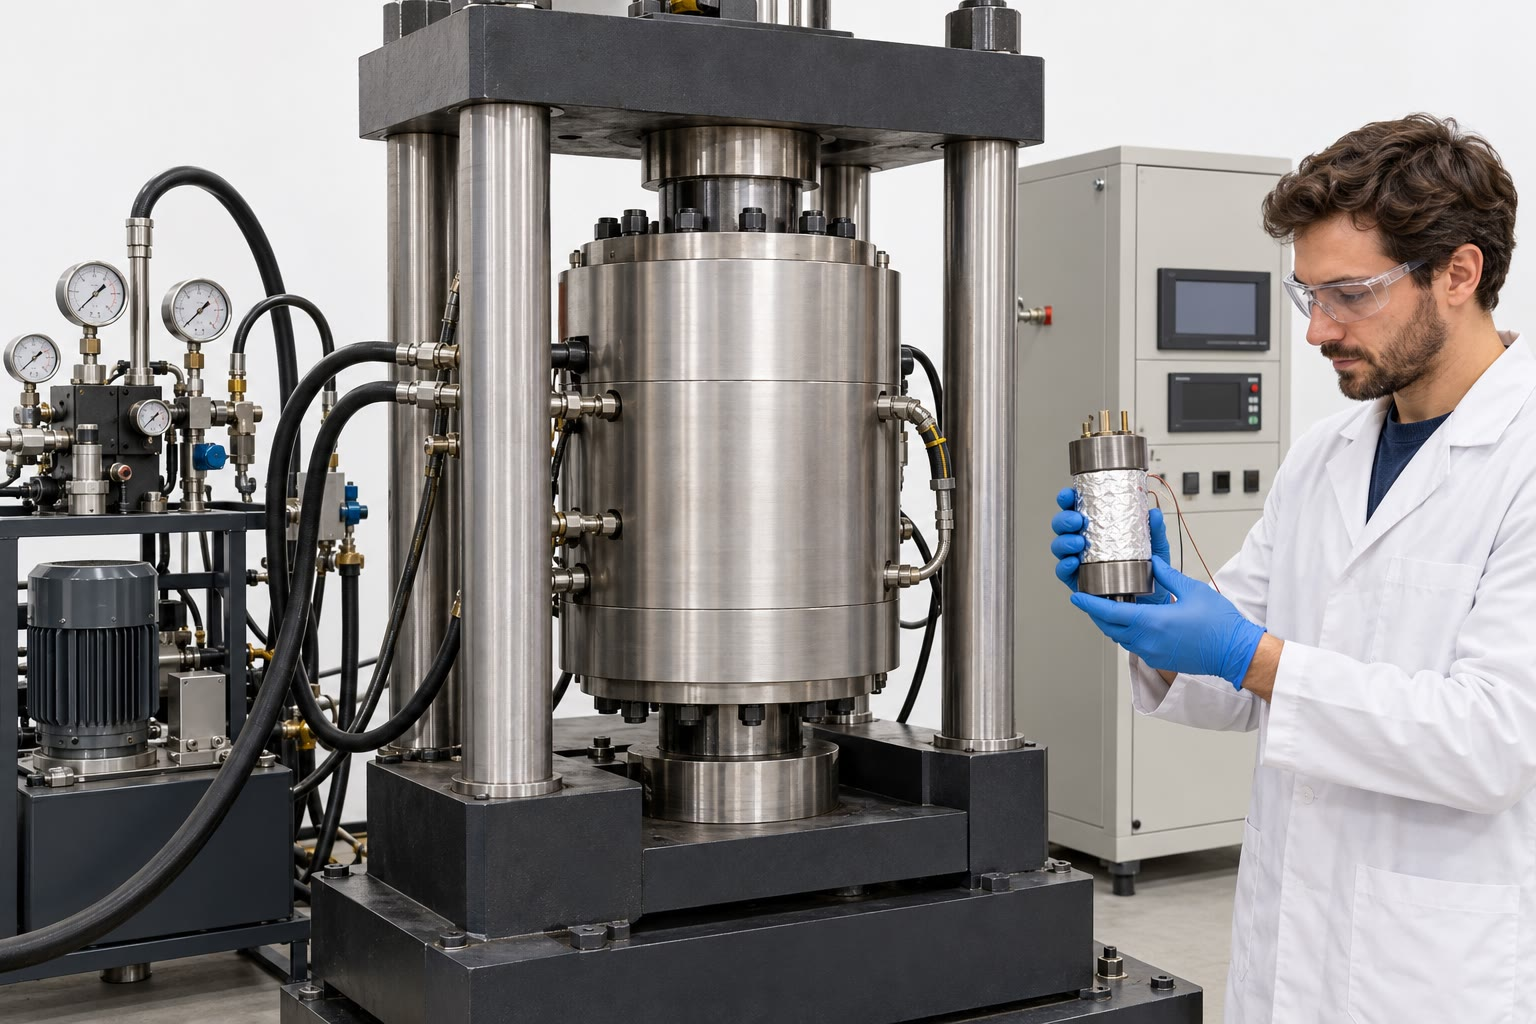
\includegraphics[width=\linewidth]{images/book5/ai/b3-deformation-press.jpg}

{\scriptsize A rock-deformation press with a jacketed sample assembly
(AI-generated illustration).}

\smallskip
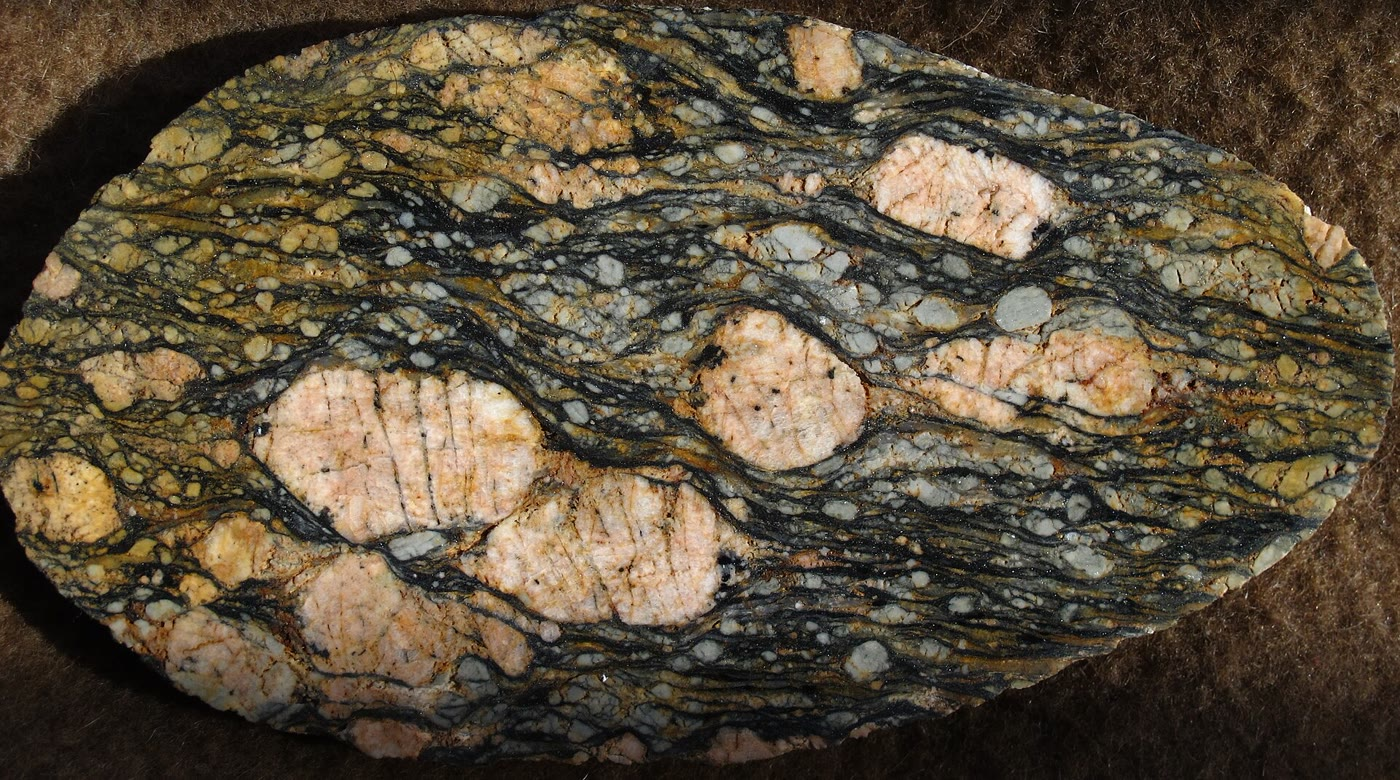
\includegraphics[width=\linewidth]{images/book5/b3-augen-mylonite.jpg}

{\scriptsize A sawn augen mylonite from Norway: large feldspar porphyroclasts
in a fine matrix of recrystallised quartz, feldspar and micas. Photo
Mikenorton, CC BY-SA 4.0.}
\end{minipage}
\end{inthelab}
% ledger: mk00:diffusion, photo:b3-augen-mylonite

\section{Exercises}

\begin{exercise}[$\star$]\label{exo:b3:deformation-mechanisms:1}
Forsterite melts at \qty{1890}{\celsius} and ice at \qty{0}{\celsius}. Compute
the \omterm{def:b3:deformation-mechanisms:flow-law}{homologous temperature} of forsterite at \qty{1300}{\celsius} and of ice at
\qty{-10}{\celsius}. Which creeps more readily?
\end{exercise}

\begin{exercise}[$\star$]\label{exo:b3:deformation-mechanisms:2}
A dyke crossing a \omterm{def:b3:deformation-mechanisms:shear-zone}{shear zone} at right angles is deflected inside the zone by
\ang{70}, and another by \ang{80}. Compute the shear strains. Why are large
strains hard to measure this way?
\end{exercise}

\begin{exercise}[$\star$]\label{exo:b3:deformation-mechanisms:3}
With the quartz piezometer, what stress does a recrystallised grain size of
\qty{10}{\micro m} indicate?
\end{exercise}

\begin{exercise}[$\star$]\label{exo:b3:deformation-mechanisms:4}
With the \omterm{def:b3:deformation-mechanisms:flow-law}{flow law} of wet quartzite ($A = \num{1.1e-4}$, $n = 4$, $E =
\qty{223}{kJ.mol^{-1}}$, $R = \qty{8.314}{J.mol^{-1}.K^{-1}}$), compute the
strain rate at \qty{500}{\celsius} under \qty{20}{MPa}.
\end{exercise}

\begin{exercise}[$\star\star$]\label{exo:b3:deformation-mechanisms:5}
Compute the effective viscosity of wet quartzite flowing at \qty{e-14}{s^{-1}}
at \qty{400}{\celsius} (\qty{65.4}{MPa}) and at \qty{500}{\celsius}
(\qty{18.0}{MPa}). Compare with the mantle viscosities of
\cref{ch:b3:mantle-convection}.
\end{exercise}

\begin{exercise}[$\star\star$]\label{exo:b3:deformation-mechanisms:6}
Two experiments at the same temperature give \qty{e-5}{s^{-1}} under
\qty{100}{MPa} and \qty{1.6e-4}{s^{-1}} under \qty{200}{MPa}. Compute the \omterm{def:b3:deformation-mechanisms:flow-law}{stress
exponent} and name the likely mechanism.
\end{exercise}

\begin{exercise}[$\star\star$]\label{exo:b3:deformation-mechanisms:7}
At the same stress, a sample creeps ten times faster at \qty{1100}{K} than at
\qty{1000}{K}. Compute the activation energy.
\end{exercise}

\begin{exercise}[$\star\star$]\label{exo:b3:deformation-mechanisms:8}
By what factor does the strain rate of \omterm{def:b3:deformation-mechanisms:creep}{diffusion creep} change when the grain
size is divided by ten, for Nabarro--Herring and for Coble creep? Why is Coble
creep the more sensitive?
\end{exercise}

\begin{exercise}[$\star\star$]\label{exo:b3:deformation-mechanisms:9}
For dry olivine at \qty{1100}{\celsius} and \qty{2}{GPa}, the two \omterm{def:b3:deformation-mechanisms:flow-law}{flow laws} give
$\dot\varepsilon_{\mathrm{dis}} = \num{6.54e-17}\,\sigma^{3.5}$ and
$\dot\varepsilon_{\mathrm{dif}} = \num{3.59e-6}\,\sigma d^{-3}$ (units of the
text). Compute the boundary stress for $d = \qty{1}{mm}$ and $d =
\qty{100}{\micro m}$, and the slope of the boundary.
\end{exercise}

\begin{exercise}[$\star\star\star$]\label{exo:b3:deformation-mechanisms:10}
Following the proof of \cref{prop:b3:deformation-mechanisms:grain-size},
explain why the lattice path gives $d^{-2}$ and the boundary path $d^{-3}$, and
show that boundary diffusion wins below the grain size $d^* \approx
(B_B/B_L)\,\delta D_B/D_L$.
\end{exercise}

\begin{exercise}[$\star\star\star$]\label{exo:b3:deformation-mechanisms:11}
For a \omterm{def:b3:deformation-mechanisms:flow-law}{flow law} with $n = 3.5$, by what factor does the effective viscosity fall
when the strain rate is multiplied by ten? Why does this favour the
localisation of strain into \omterm{def:b3:deformation-mechanisms:shear-zone}{shear zones}?
\end{exercise}

\begin{exercise}[$\star\star\star$]\label{exo:b3:deformation-mechanisms:12}
In the dry olivine of exercise 9, a mantle \omterm{def:b3:deformation-mechanisms:shear-zone}{shear zone} under \qty{10}{MPa}
recrystallises from \qty{3}{mm} to \qty{30}{\micro m} grains. Compute the total
strain rate before and after, and the factor of softening. Which mechanism
carries the deformation in each case?
\end{exercise}

\section{Problem: The Varden Shear Zone}

\begin{problem}[{Weekend problem --- the strain, stress, strain rate and age
of an invented shear zone}]
\label{pb:b3:deformation-mechanisms:1}
% values: calc/ch07.py; flow_laws.py; st03:piezometer, lopez:flow-laws
Beneath the granite of the Varden Hills, the series' invented region, a
borehole and a deep road cut (both invented) reveal a ductile \omterm{def:b3:deformation-mechanisms:shear-zone}{shear zone}
\qty{400}{m} wide, formed at about \qty{15}{km} depth and \qty{450}{\celsius}.
A dolerite dyke that crosses the walls at right angles makes, inside the zone,
an angle of only \ang{6} with the zone's boundaries. Its quartz is a mylonite
of recrystallised grains \qty{20}{\micro m} across (from 15 to
\qty{25}{\micro m}). Take the quartz piezometer $D = 10^{3.56}\sigma^{-1.26}$,
the \omterm{def:b3:deformation-mechanisms:flow-law}{flow law} of wet quartzite ($A = \num{1.1e-4}$, $n = 4$, $E =
\qty{223}{kJ.mol^{-1}}$), $R = \qty{8.314}{J.mol^{-1}.K^{-1}}$, \qty{1}{yr} $=
\qty{3.156e7}{s}$, and, in simple shear, $\dot\gamma = 2\dot\varepsilon$.

\medskip\noindent\textbf{Part I --- The strain.}
\begin{enumerate}
  \item Compute the deflection $\psi$ of the dyke and the shear strain.
  \item Compute the displacement of one wall relative to the other.
  \item Compute the principal stretches of the strain ellipse and its axial
        ratio.
  \item Compute the angle of the long axis with the zone. What does the
        foliation of the zone do as $\gamma$ grows?
  \item Seen from above, the dyke, followed from the southern wall, bends to
        the east as it enters the east--west zone, then returns to its
        northward course at the northern wall. Which way did the northern wall
        move, and is the zone dextral or sinistral?
  \item In which plane should a thin section be cut to read the \omterm{def:b3:deformation-mechanisms:kinematic}{kinematic
        indicators}, and how should its S foliation lean?
\end{enumerate}

\medskip\noindent\textbf{Part II --- The stress.}
\begin{enumerate}[resume]
  \item Compute the stress indicated by the \qty{20}{\micro m} grains.
  \item Compute the stresses for 15 and \qty{25}{\micro m}.
  \item Is the stress within the range of the calibration?
  \item The piezometer showed no effect of temperature. Why does this matter
        here?
  \item What grain size would a stress of \qty{100}{MPa} have produced?
\end{enumerate}

\medskip\noindent\textbf{Part III --- The strain rate.}
\begin{enumerate}[resume]
  \item Compute $E/RT$ at \qty{450}{\celsius} and the Arrhenius factor.
  \item Compute the strain rate of the quartz under the stress of question 7
        (take \qty{62}{MPa}).
  \item Compute the shear strain rate.
  \item Compute the effective viscosity of the zone and compare it with the
        upper mantle of \cref{ch:b3:mantle-convection}.
  \item By what factors would the strain rate change at 400 and
        \qty{500}{\celsius}, at the same stress?
  \item By what factor if the stress were the \qty{78}{MPa} of the finest
        grains?
\end{enumerate}

\medskip\noindent\textbf{Part IV --- The time.}
\begin{enumerate}[resume]
  \item Compute the time needed to accumulate the shear strain of question 1,
        in seconds.
  \item Convert it to thousands of years.
  \item Compute the mean slip rate across the zone, in \unit{mm/yr}.
  \item Compare it with plate-boundary rates of tens of millimetres a year.
        % ledger: morvel:range
  \item If the zone had carried \qty{20}{mm/yr}, what shear strain rate, stress
        and recrystallised grain size would it have had?
  \item How do the uncertainties of the grain size and of the piezometer's
        exponent affect the time?
  \item Give the time the Varden \omterm{def:b3:deformation-mechanisms:shear-zone}{shear zone} took to accumulate its strain, in
        thousands of years.
\end{enumerate}
\end{problem}
